\documentclass{scrartcl}
\usepackage{graphicx}
\usepackage{hyperref}
\usepackage{tikz}
\usepackage{xcolor}
\usepackage{amsmath}


\usetikzlibrary{shapes}
\usetikzlibrary{positioning}





% Title Page
\title{Master Thesis}
\subtitle{A Remotely-driven Hoverboard With Platform Leaning Control}

\author{Author: Esteve Tarrag\'o \\
	Advisors: Llu\'is Ros \ Enric Celaya\\
	Tutor: Merc\`e Oll\'e\\
	MSc in Advanced Mathematics and Mathematical Engineering\\
	Institut de Robòtica i Informàtica Industrial
}
\begin{document}
\maketitle

\newpage
\begin{abstract}
	TO DO: This is the abstract
\end{abstract}

\newpage
\tableofcontents

\section{Introduction}
In the IRI lab we have two segway robots, Tibi and Dabo show in figure
\ref{fig:Picture of Tibi and Dabo}. Both of them move the same way.
They must incline their body to compensate the wheel reaction. 
This may cause some problems when measuring distances with the sensors.
This fact also restricts the possible trajectories of the robots. 

We decided to build a prototype of segway robot that could control it's
inclination independently. The chosen robot is inspired in a \textit{segway hover-board}, 
similar to the one appearing in Figure \ref{fig:Picture of a commercial 
segway hover-board}. The two wheels are controlled with classic
control algorithms and the inclination of the central body is
controlled with a flywheel mechanism that we will discuss in section \ref{}.

\begin{figure}
	\centering
	\includegraphics[width=8cm]{img/robots-TIBI-i-DABO-IRI-red.jpg}
	\caption{Picture of Tibi and Dabo, \textit{two segway robots} }
	\label{fig:Picture of Tibi and Dabo}
\end{figure}

\begin{figure}
	\centering
	\includegraphics[width=8cm]{img/segway_hoverboard_picture.png}
	\caption{Picture of a commercial \textit{segway hover-board} }
	\label{fig:Picture of a commercial segway hover-board}
\end{figure}

\section{Initial design considerations}
The first thing we decided is the number of actuators.
Most of segway robot include two motors for the motion control but we added a third on in order to control the inclination.
We included three motors in total because we want to control three degrees of freedom (inclination and speed of both wheels).

In order to control the inclination of the platform we needed to add an external torque to the platform. We considered three methods: accelerating a flywheel, holding a pendulum in a non-vertical position and air friction with a fan. We discarded the last one due to the high speeds we needed to obtain a reasonable torque on the platform.

Both methods have strengths in different situations so we decided to build a mixed method that could combine both. 


We took two restriction in our design. The first one symmetry along the inclination axis in order to have an equilibrium in all possible inclinations without the need of external forces. We also took in consideration that the reinforcement learning algorithms starts being clumsy so none of the configurations should touch the ground. Figure \ref{fig:Side render view} illustrates this restriction.   

The design of the robot is done with the 3D design software \href{https://www.freecadweb.org/}{Free-cad}. All part files are uploaded to the GitHub repository \url{https://github.com/tarragoesteve/TFM} under the hardware folder.

You can see the main views on Figure \ref{fig:Isometric render view}, \ref{fig:Front render view}, \ref{fig:Top render view} and \ref{fig:Side render view}.

\begin{figure}
	\centering
	\includegraphics[width=10cm]{img/isometric_view.png}
	\caption{Isometric render view}
	\label{fig:Isometric render view}
\end{figure}
\begin{figure}
	\centering
	\includegraphics[width=10cm]{img/front_view.png}
	\caption{Front render view}
	\label{fig:Front render view}
\end{figure}
\begin{figure}
	\centering
	\includegraphics[width=10cm]{img/top_view.png}
	\caption{Top render view}
	\label{fig:Top render view}
\end{figure}
\begin{figure}
	\centering
	\includegraphics[width=4cm]{img/side_view.png}
	\caption{Side render view}
	\label{fig:Side render view}
\end{figure}

\subsection{Flywheel design}
\begin{figure}
	\centering
	\includegraphics[width=5cm]{img/fly_wheel_side.png}
	\caption{Fly wheel side render view}
	\label{fig:Fly wheel side render view}
\end{figure}

To control the inclination of the body two strategies are taken in to account. Creating torque by a pendulum or accelerating the flywheel. In order to experiment with both of them we designed a part to allow both configuration by placing weights in different spots, see figure \ref{fig:Fly wheel side render view}.

In order to create a configuration with maximum gravitational torque we have done the following computation. We denote the torque pendulum torque $\tau$, consider the masses are cylinders of mass $m_{cylinder}$ with radius $r_c$ and width $w$ and the radius of the flywheel is $r_f$.

Each mass weights:
\[ m_{cylinder} = \rho * w * \pi * r_c^2 \]

We neglect the mass of the flywheel structure versus the mass of the cylinders so all the gravitational torque created by the masses will be compensated with the opposite weight except for the two masses with different radius.

One of the weight can be placed along a rail. The distance to the center will vary from $r_{min} = r_c + r_{motor-axis} \approx r_c $ to $r_{max} = r_f - r_c$. 

The maximum torque takes place when these two masses are aligned horizontal with respect the ground and the movable weight is at distance $r_{min}$ from the center.

\[ \tau _{max} (r_c) =  m_{cylinder} * g * r_{max} -  m_{cylinder} * g * r_{min} =  m_{cylinder}* g * (r_f - 2 * r_c) \]

In order to maximize $\tau$ it we first compute the derivative:
\[\frac{\partial \tau _{max} (r_c)}{\partial r_c} = g *(\frac{\partial m}{\partial r_c} * (r_f - 2 * r_c) -  m_{cylinder} * 2)\]

\[ \frac{\partial  m_{cylinder}}{\partial r_c} = 2 * \rho * w * \pi *  r_c\]

An make it zero to find the maximum:

\[\frac{\partial \tau _{max} (r_c)}{\partial r_c} = 0\]

Substituting and simplifying we get:

\[\frac{\partial m}{\partial r_c} * (r_f - 2 * r_c) =   m_{cylinder} * 2 \Rightarrow 2 * \rho * w * \pi *  r_c\ * (r_f - 2 * r_c) = \rho * w * \pi * r_c^2 * 2 \]

\[ \Rightarrow r_c\ * (r_f - 2 * r_c) =  r_c^2 \Rightarrow (r_f - 2 * r_c) =  r_c \Rightarrow \boxed{r_f = 3 * r_c}\]


The circumradius $R$ from the center of a regular polygon to one of the vertices is related to the side length $s$ by:

\begin{center}
	\begin{tabular}{ c  c }
		\(\displaystyle R=\frac {s}{2* \sin{\frac {\pi} {n}}} \)
		& 
		\includegraphics[width=3cm]{img/PolygonParameters.png}
	\end{tabular}
\end{center}

In our case:
\[ R = r_f - r_c; \]
\[ s = 2 * r_c\]

Substituting in the circumradius equation we get n = 6, so we will use up 6 masses in our flywheel.
We will have a variable number of masses $N$ that we will be able to add to the flywheel as shown in the following table.
\begin{center}
	\begin{tabular}{c | c | c | c }
	 2 & 3 & 4 & 6 \\
	 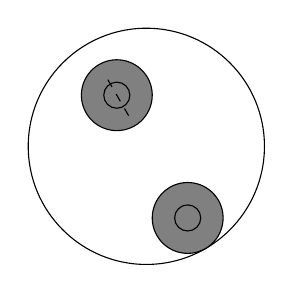
\begin{tikzpicture}[scale=0.5]
		%Circle
			\path node (center) at (0,0) {};
			\draw (center) circle (3);
		%Movable mass
			\draw[rotate=120,fill=gray] (1.5,0) circle (.9) node (moving) [draw,circle]{};
		%Guide
			\draw[dashed,rotate=120] (.9,0) -- (2.1,0);
		%Other masses
			\foreach \i in {2}
			{
				\draw[rotate=60-60*\i,fill=gray] (3-.9,0) circle (.9) node[draw,circle]{};
			}
	\end{tikzpicture}
	
	 & 
	 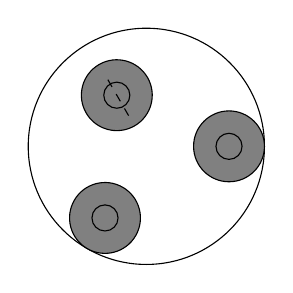
\begin{tikzpicture}[scale=0.5]
		%Circle
			\path node (center) at (0,0) {};
			\draw (center) circle (3);
		%Movable mass
			\draw[rotate=120,fill=gray] (1.5,0) circle (.9) node (moving) [draw,circle]{};
		%Guide
			\draw[dashed,rotate=120] (.9,0) -- (2.1,0);
		%Other masses
			\foreach \i in {1,3}
			{
				\draw[rotate=60-60*\i,fill=gray] (3-.9,0) circle (.9) node[draw,circle]{};
			}
	\end{tikzpicture}
	 & 
	 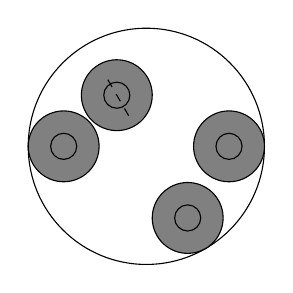
\begin{tikzpicture}[scale=0.5]
		%Circle
			\path node (center) at (0,0) {};
			\draw (center) circle (3);
		%Movable mass
			\draw[rotate=120,fill=gray] (1.5,0) circle (.9) node (moving) [draw,circle]{};
		%Guide
			\draw[dashed,rotate=120] (.9,0) -- (2.1,0);
		%Other masses
			\foreach \i in {1,2,4}
			{
				\draw[rotate=60-60*\i,fill=gray] (3-.9,0) circle (.9) node[draw,circle]{};
			}
	\end{tikzpicture} 
	&
	
	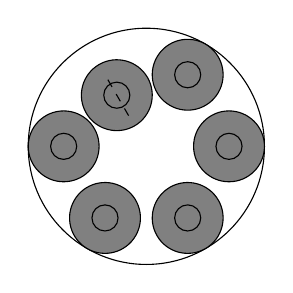
\begin{tikzpicture}[scale=0.5]
		%Circle
			\path node (center) at (0,0) {};
			\draw (center) circle (3);
		%Movable mass
			\draw[rotate=120,fill=gray] (1.5,0) circle (.9) node (moving) [draw,circle]{};
		%Guide
			\draw[dashed,rotate=120] (.9,0) -- (2.1,0);
		%Other masses
			\foreach \i in {1,2,3,4,6}
			{
				\draw[rotate=60-60*\i,fill=gray] (3-.9,0) circle (.9) node[draw,circle]{};
			}
	\end{tikzpicture}
	\\  
	\end{tabular}
	\end{center}

\section{Mechanical analysis}
\subsection{Reference frames}
In order to study the behavior of the robot we will use the following frames:
\begin{itemize}
    \item Absolute frame: From a fix object in the room. 
    \item Body frame: From the body of our robot.
\end{itemize}

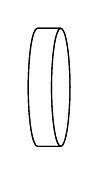
\begin{tikzpicture}[]
    \node (left_wheel) [cylinder, shape border rotate=0, draw, minimum height=1mm, minimum width=15mm] {};

    \node (right_wheel) [cylinder, shape border rotate=0, draw, minimum height=1mm, minimum width=15mm] {};

    \coordinate (left_wheel 0 0);
    \coordinate (right_wheel 10 0);



    \end{tikzpicture}


\subsection{Inclination control}
In order to keep the inclination at a certain angle we must be able to compensate all the torque being applied to the body.

Assuming that the body is well balanced and neglecting the torque generated by the friction with air, the sum of all the torques in the motor axis applied to the body is equal to the sum of the torque applied by the motors:

\[\tau_{body} = \sum \tau_{motors}\]

The torque of the motors produce a reaction in the body opposite to the torque that the motors deliver to the wheels and the flywheel.

\[\tau_{body} = -\tau_{right-wheel} -\tau_{left-wheel} -\tau_{flywheel} \]

If we want to control the inclination $\theta$, we must be able to control $\tau_{body}$ in a range $\tau_{body} \in (-\epsilon, \epsilon)$. Observe that the angular acceleration of the body is linearly dependent with the torque it receives. In the limit case $\epsilon = 0$. In order to simplify the calculations we will assume $\epsilon = 0$.

\[0 = -\tau_{right-wheel} -\tau_{left-wheel} -\tau_{flywheel} \Rightarrow \tau_{right-wheel} +\tau_{left-wheel} = -\tau_{flywheel} \]

In other words, we must compensate the torque of the wheels with the torque of the flywheel.

\subsection{Wheels torque}
The wheel torque we can induce is limited by the motor specifications. Note that the maximum torque of the motor is a function of velocity and in particular at max speed the torque is zero.

\[\tau_{motor} (w_{wheel}) \]


We assume that the wheels just roll and do no slip.
The robot is pushed by the wheels that make a force $F_{drag}$ against the ground in the contact point. See figure \ref{fig:Wheel force diagram}.

We can express the torque of the wheel as:
\[ \tau_{wheel} =min(\tau_{motor} (w_{wheel}), I_{wheel} * \dot{w}_{wheel} - F_{drag} * r_{wheel})\]
\begin{figure}[ht]
	\centering
	\includegraphics[width=10cm]{img/wheel_diagram.jpg}
	\caption{Wheel force diagram}
	\label{fig:Wheel force diagram}
\end{figure}


\subsection{Flywheel torque}

\begin{figure}
	\centering
	\includegraphics[width=10cm]{img/flywheel_diagram.jpg}
	\caption{Flywheel force diagram}
	\label{fig:Flywheel force diagram}
\end{figure}

The flywheel torque we can induce is also limited by the motor specifications. 

Assuming that a general configuration of the flywheel, see figure \ref{fig:Flywheel force diagram}. we formulate its torque the following way:


\[\tau_{flywheel} = min(\tau_{motor} (w), \ddot{\theta}*I_{flywheel}(r) + m_{cylinder} * g * (r - r_{max}) * \sin{\theta}) \]

\subsection{Motor specifications}

Here we have the factory specifications of our motors: 
\begin{itemize}
    \item Operating voltage: between 3 V and 9 V
    \item Nominal voltage: 6 V
    \item Free-run speed at 6 V: 176 RPM
    \item Free-run current at 6 V: 80 mA
    \item Stall current at 6V: 900 mA
    \item Stall torque at 6V: 5 kg·cm
    \item Gear ratio: 1:35
    \item Reductor size: 21 mm
    \item Weight: 85 g
\end{itemize}

\subsection{Hypothesis}
Assuming that the body is well balanced

\section{Optimization Setup}
In this section we will set up the requirements and the cost function we want to optimize.

\subsection{Restrictions}
The restrictions are a list of inequalities that our system has to fulfill.
The first restriction is due to the initial design requirements. Finally, the other three are 
somehow arbitrary but will help us to reduce the size of the robot.
\begin{enumerate}
\item We will place our flywheel in a hole on our robot. We don't want to touch the ground
in any configuration so:
\begin{figure}[ht]
	\centering
	\includegraphics[width=7cm]{img/flywheel_hole.jpg}
	\caption{Flywheel hole diagram}
	\label{fig:Flywheel hole diagram}
\end{figure}
\[r_{wheel}> \sqrt{(r_{flywheel} + b)^2+(\frac{h}{2})^2}\]
\item Being able  to insert the robot in to a wheel of diameter 0.5 m so:
\begin{figure}[ht]
	\centering
	\includegraphics[width=7cm]{img/external_diameter.jpg}
	\caption{External diameter diagram}
	\label{fig:External diameter diagram}
\end{figure}
\[0.25 m > \sqrt{r_{wheel}^2 + L^2/4}\]
\item We can place all electronic the devices:
\[L > 0.3m + w \]
\item Maximum weight of the robot: 5 kg
\end{enumerate}

\subsection{Requirements}
We would like our robot to reach some mechanical specifications. These are related to mechanical equations
that we will develop in the next section. They refer to the max speed, acceleration and terrain inclination the robot may achieve
while controlling its platform inclination. We have divided our specifications in two blocks
according to the two mechanisms.

\textbf{Flywheel mode}
\begin{enumerate}
	\item $\dot{y}_{max}$ (equation \ref{Maximum speed flywheel}) $> 0.1m/s$.
	\item $\ddot{y}_{max}$ (equation \ref{maximum acceleration flywheel}) $> 1m/s^2$.
	\item $sin(\alpha_{max})$ (equation \ref{Maximum angle using flywheel system}) $>0.16$.
\end{enumerate}

\textbf{Pendulum mode}
\begin{enumerate}
	\item $\dot{y}_{max}$ (equation \ref{maximum speed pendulum}) $>1m/s$.
	\item $\ddot{y}_{max}$ (equation \ref{maximum acceleration pendulum}) $>0.1m/s^2$.
	\item $sin(\alpha_{max})$ (equation \ref{Maximum angle using pendulum system}) $> 0.02$.
\end{enumerate}
	


\subsection{Cost function}
In addition to fulfilling the previous inequalities, we will adjust our design parameters [w (width of the
cylinders), N(number of cylinders), r wheel and r flywheel] to
minimize a cost function. 

We will maximize the maximum sinus in the pendulum mode 
(equation \ref{Maximum angle using pendulum system}) because
it gives the robot the capacity to deliver force in a permanent state.

And we will also maximize the square of the max speed the robot can achieve
in flywheel mode (equation \ref{Maximum speed flywheel}) because it is
proportional to the energy the robot can deliver using the flywheel at a certain moment.

Both equations try to maximize different modes so the robot we have a compromise between the two of them. 

\begin{equation}
	cost(r_{flywheel},r_{wheel},w,N) = - sin(\alpha_{max})_{pendulum} -\dot{y}^2_{max-flywheel}
	\label{eq: cost}
\end{equation}
In the next section we will find out what are the values 
of these equations with the construction parameters. 
%For reference these terms are equal to:
%\begin{equation*}
%	m_{cylinder} = \rho * w * \pi * (\frac{r_{flywheel}}{3})^2
%\end{equation*}
%\begin{equation*}
%	sin(\alpha_{max})_{pendulum} = \frac{m_{cylinder} \cdot  (r_{max} - r_{min})}{m_{total} \cdot r_{wheel}} = \frac{m_{cylinder} \cdot  (\frac{r_{flywheel}}{3})}{(m_{rest} + N \cdot m_{cylinder})\cdot r_{wheel}} 	
%\end{equation*}
%\begin{equation*}
%	\dot{y}_{max} = r_{wheel} \cdot  R \cdot  \dot{\theta}_{max} =r_{wheel} \cdot  \frac{ N \cdot  m_{cylinder} \cdot  (\frac{2\cdot r_{flywheel}}{3})^2}
%    {r_{wheel}^2\cdot (m_{rest} + N \cdot m_{cylinder}) +  2\cdot I_{wheel}} \cdot  \dot{\theta}_{max}
%\end{equation*}

\section{Flywheel break study}

This section aims to study a possible way to break the flywheel without applying torque to the platform. The idea is the following: we will leave the moving weight free.

This way, when the weight is going upward will have a larger radius than when is going downward and will produce an average moment against the movement of the flywheel.

From an energetic point of view we are transforming the rotation energy of the flywheel in to translation of the free cylinder and then realising it trough collisions.
\subsection{System of differential equations}
As described in figure \ref{fig:Flywheel force diagram} we will use two variables to describe the flywheel position: $r$, $\theta$ 

Using equation \ref{flywheel equation}:
\[\tau_{flywheel} = -\ddot{\theta}*I_{flywheel}(r) + m_{cylinder} * g * (r - r_{max}) * \sin{\theta}\]
\begin{figure}[ht]
	\centering
	\includegraphics[width=10cm]{img/cylinder_forces.png}
	\caption{Cylinder force diagram}
	\label{fig:Cylinder force diagram}
\end{figure}

As seen in figure \ref{fig:Cylinder force diagram}, we can deduce newtons equation for the distance from the cylinder to the center $r$. Note that we are adding the centrifugal force term due to the non-inertial frame.
\[\ddot{r} * m = -m * g * sin(\pi/2-\theta) + m * r * \dot{\theta}^2 \]
\[\ddot{r} = -g * sin(\pi/2-\theta) + r * \dot{\theta}^2 \]

The variables we will be using for our ODE system are: $r$,$\dot{r}$,$\theta$,$\dot{\theta}$

Note that we impose $\tau_{flywheel} = 0$ so the motor is not applying any torque.

\[
\begin{cases}
    \dot{r} = \dot{r}\\
    \ddot{r} = -g * sin(\pi/2-\theta) + r * \dot{\theta}^2\\
    \dot{\theta} = \dot{\theta}\\
    \ddot{\theta} = \frac{m_{cylinder} * g * (r - r_{max}) * \sin{\theta}}{I_{flywheel}(r)} \\    
\end{cases}
\]


Our initial conditions will be the free cylinder mass lying on the bottom of the flywheel and the flywheel turning at a speed $\theta_0$:
\[
    \begin{cases}
        r = r_{max} \\
        \dot{r} = 0\\
        \theta = \pi\\
        \dot{\theta} = \theta_0\\
    \end{cases}
\]

We will use a poincare map to simulate the bounce with the end of the guides at $r=r_{min}$ and $r=r_{max}$. At each bounce we will reduce its kinetic energy by a percentage $bounce\_percentage$ .

\subsection{Results}
The parameters of the simulation where:
\[
\begin{cases}
	r_{flywheel} = 5cm \\
	r_{wheel} = 7cm \\
	w = 2 cm \\
	\dot{\theta}_0 = 5 \pi rad/s \\
	bounce\_percentage = 0.1 \\	
\end{cases}	
\]

As we can see in figure \ref{fig:d theta t diagram} the flywheel is breaking until it becomes a pendulum and starts oscillating.

\begin{figure}[ht]
	\centering
	\includegraphics[width=10cm]{img/simulation/r_t.png}
	\caption{How the variable $r$ evolves over time}
	\label{fig:r t diagram}
\end{figure}

\begin{figure}[ht]
	\centering
	\includegraphics[width=10cm]{img/simulation/theta_t.png}
	\caption{How the variable $\theta$ evolves over time}
	\label{fig:theta t diagram}
\end{figure}

\begin{figure}[ht]
	\centering
	\includegraphics[width=10cm]{img/simulation/r_theta_t.png}
	\caption{How the variable $r$ evolves over $\theta$}
	\label{fig:r theta}
\end{figure}

\begin{figure}[ht]
	\centering
	\includegraphics[width=10cm]{img/simulation/r_theta_t_zoom.png}
	\caption{How the variable $r$ evolve over $\theta$}
	\label{fig:r theta zoom}
\end{figure}

\begin{figure}[ht]
	\centering
	\includegraphics[width=10cm]{img/simulation/d_theta_t.png}
	\caption{How the variable $\dot{\theta}$ evolve over time}
	\label{fig:d theta t diagram}
\end{figure}


\end{document}          
